% !TEX encoding = UTF-8 Unicode

\documentclass[12pt,reqno]{amsart}
\usepackage[russian]{babel}
\usepackage[utf8]{inputenc}
%\usepackage[dvips]{graphicx,graphics}
\usepackage{graphicx}
\usepackage{euscript}
\usepackage{graphics}
%\usepackage{russcorr}
\usepackage[active]{srcltx} % SRC Specials: DVI [Inverse] Search
\usepackage{amssymb,amsmath,amsthm,amsfonts}
\usepackage{amsopn}
\newtheorem{cor}{Следствие}
\newtheorem{lem}{Лемма}
\newtheorem{thm}{Теорема}
\newtheorem{prop}{Предложение}
\newtheorem*{thm_pres}{Теорема}
\theoremstyle{definition}
\newtheorem{defn}{Определение}
\newtheorem{defneq}{Эквивалентное определение}
\theoremstyle{remark}
\newtheorem*{rem}{Замечание}
\newtheorem*{deff}{Обозначение}
\usepackage{verbatim}
\usepackage{listings}
\usepackage{hyperref}
\usepackage{color}

\definecolor{dkgreen}{rgb}{0,0.6,0}
\definecolor{gray}{rgb}{0.5,0.5,0.5}
\definecolor{mauve}{rgb}{0.58,0,0.82}

\lstset{frame=tb,
  language=Java,
  aboveskip=3mm,
  belowskip=3mm,
  showstringspaces=false,
  columns=flexible,
  basicstyle={\small\ttfamily},
  numbers=none,
  numberstyle=\tiny\color{gray},
  keywordstyle=\color{blue},
  commentstyle=\color{dkgreen},
  stringstyle=\color{mauve},
  breaklines=true,
  breakatwhitespace=true,
  tabsize=3
}

\newcommand{\sug}[1]{\rule[-2mm]{0.4pt}{5mm}_{\,{#1}}}
\newcommand{\gen} {$GE^+_n(\mathbf{R}[x])\ $}
\newcommand{\genn} {$GE^+_2(\mathbf{R}[x])\ $}
\newcommand{\gn} {$G_n(\mathbf{R})\ $}
\newcommand{\gln} {$GL_n(\mathbf{R}[x])\ $}
\newcommand{\p} {\mathbf{P}}
\newcommand{\peq} {$\mathcal{P}$}
\newcommand{\po} {$\mathcal{P}_0$}
\newcommand{\ff} {$\mathbf{R}\ $}
\newcommand{\fx} {\mathbf{R}[x]}
\newcommand{\fp} {\mathbf{R_+}}
\newcommand{\fxp} {\mathbf{R_+}[x]}
\newcommand{\zx} {\mathbb{Z}[x]}
\newcommand{\zxp} {\mathbb{Z_+}[x]}
\newcommand{\basering} {$\mathbf{F}$}
\newcommand{\lfrac} [2] {\displaystyle \frac{#1}{#2}}
\newcommand{\brsum} [3] {\displaystyle \sum \limits_{#1}^{#2} \left( #3\right)}
\newcommand{\lsum} [2] {\displaystyle \sum \limits_{#1}^{#2}}
\newcommand{\br} [1] {\left( #1 \right)}
\newcommand{\tab} {\mbox{             } \quad }
\usepackage{a4wide}


\begin{document}
\section*{Описание метода решения задачи Коши}

Для решения задачи Коши от двух переменных выбран метод Эйлера. Он заключается в том, что мы строим точки $x_n, y_n, t_n$ по следующему индективному правилу:

 $\bullet$ $x_0, y_0$ -- начальная точка из условия задачи Коши, $t_0 = 0$,

 $\bullet$ $x_{n + 1} = x_n + t * f_x(x_n, y_n, t_n),\quad y_{n + 1} = y_n + t * f_y(x_n, y_n, t_n), \quad t_{n+1} = t_n + t$,

где $t$ -- значение временного шага. Чем оно меньше, тем точнее решение, полученное в результате применения метода.

Полученные точки $(x_n, y_n)$ образуют табулированное численное решение.

\section*{Единственность решения}

Точное решение задачи Коши единственно по теореме о единственности.

Наше численное решение для заданного заранее параметра $t$ также обладает свойством единственности, так как если бы фазовые кривые пересекались, возникло бы противоречие с тем, что для точки пересечения алгоритм построения следующей точки решения детерминирован.

\section*{Применение решения для конкретной задачи Коши}

Рассмотрим задачу $x^\prime = y,\quad y^\prime = -x, \quad x_0 = 1, \quad y_0 = 0$.

Ее точное решение: $x = cos(t), \quad y = -sin(t)$. Без заданного начального условия, фазовые кривые имеют вид $x = C \mathrm{cos}(t), \quad y = -C \mathrm{sin}(t)$, являются окружностями всех радиусов вокруг начала координат.

Код, строящий графики

\begin{lstlisting}
class DiffEq(object):
	def __init__(self, fx, fy, start_t, end_t, step_t, x0, y0):
		self.fx = fx
		self.fy = fy
		self.start_t = start_t
		self.end_t = end_t
		self.step_t = step_t
		self.x0 = x0
		self.y0 = y0

	def build_solution(self):
		x = []
		y = []
		x_y_data = []
		cur_t = self.start_t
		prev_x = self.x0
		prev_y = self.y0
		prev_t = cur_t
		while cur_t < self.end_t:
			cur_x = prev_x + (cur_t - prev_t) * self.fx(x = prev_x, y = prev_y, t = prev_t)
			cur_y = prev_y + (cur_t - prev_t) * self.fy(x = prev_x, y = prev_y, t = prev_t)
			x.append((cur_t, cur_x))
			y.append((cur_t, cur_y))
			x_y_data.append((cur_x, cur_y))
			prev_x = cur_x
			prev_y = cur_y
			prev_t = cur_t

			cur_t += self.step_t
		self.x = x
		self.y = y
		self.x_y_data = x_y_data


x = var('x')
y = var('y')
t = var('t')
g = Graphics()
g += plot_vector_field((y, -x), (x,-1.1,1.1), (y,-1.1,1.1), color="blue")
g += parametric_plot((cos(t),sin(t)),(t, 0, 2*pi),color="green")
diff_eq = DiffEq(y, -x, 0, 2*pi, 0.01, 1, 0)
diff_eq.build_solution()
g += list_plot(diff_eq.x_y_data, plotjoined=True,color="red")
g.save("diff_eq_solution.png")
\end{lstlisting}
\newpage

Синим цветом обозначено веркторное поле, зеленым -- идеальное аналитическое решение, красным -- приближенное решение. Видно, что оно отличается от идеального решения.

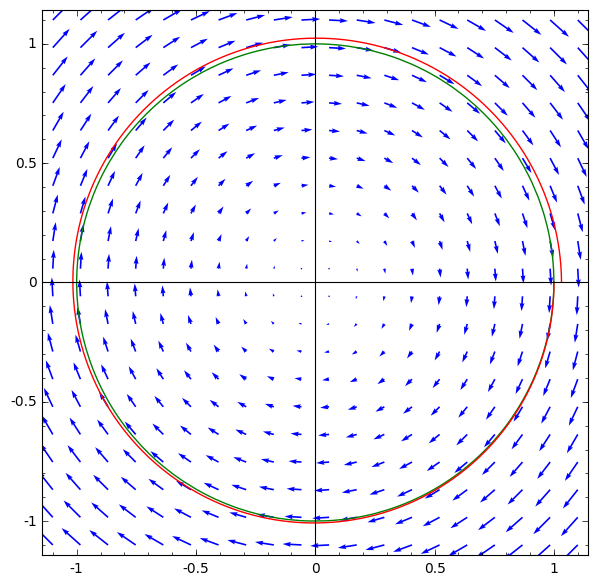
\includegraphics[width=1 \textwidth]{diff_eq_solution.png}

\section*{Оценка погрешности метода}

Для выше рассмотренной задачи построим графики логарифма ошибки по норме Чебышева от логарифма шага алгоритма.

Код, который строит график ошибки
\begin{lstlisting}
x = var('x')
y = var('y')
t = var('t')
h = 0.3
log_error_points = {}
while h > 0.01:
	diff_eq = DiffEq(y, -x, 0, 2*pi, h, 1, 0)
	diff_eq.build_solution()

	print "for h={h}".format(h=h)
	for (real_func, approx_func, var_name) in ((cos(t), diff_eq.x, 'x'), (-sin(t), diff_eq.y, 'y')):
		max_norm = 0
		cur_t = 0
		for (t_, x_) in approx_func:
			if max_norm < abs(real_func(t_) - x_):
				max_norm = abs(real_func(t_) - x_)

		log_error_points.setdefault(var_name, []).append((-log(h), log(max_norm)))

	h -= 0.01

for var_name in ('x', 'y'):
	g = Graphics()
	g += list_plot(log_error_points[var_name], plotjoined=True, legend_label="{var_name}_error".format(var_name=var_name), gridlines=True)
	g.save("diff_eq_{var_name}_error.png".format(var_name=var_name))
\end{lstlisting}

Графики ошибок:

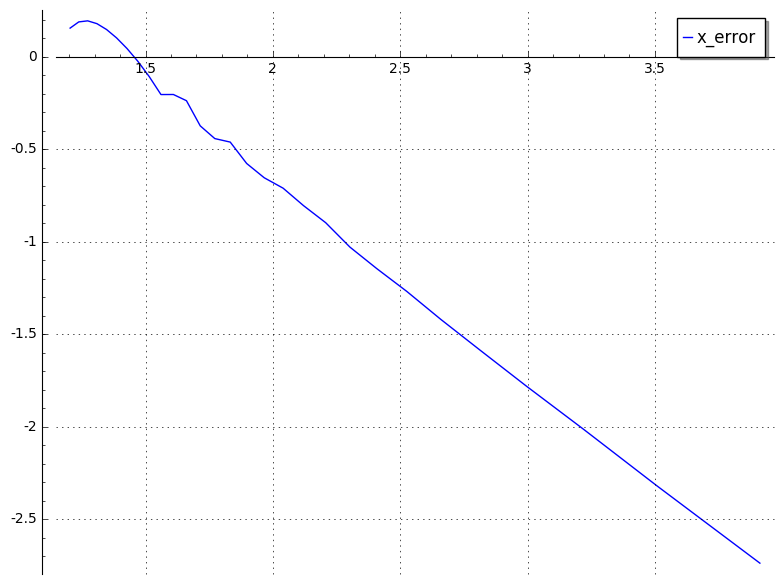
\includegraphics[width=0.4 \textwidth]{diff_eq_x_error.png}
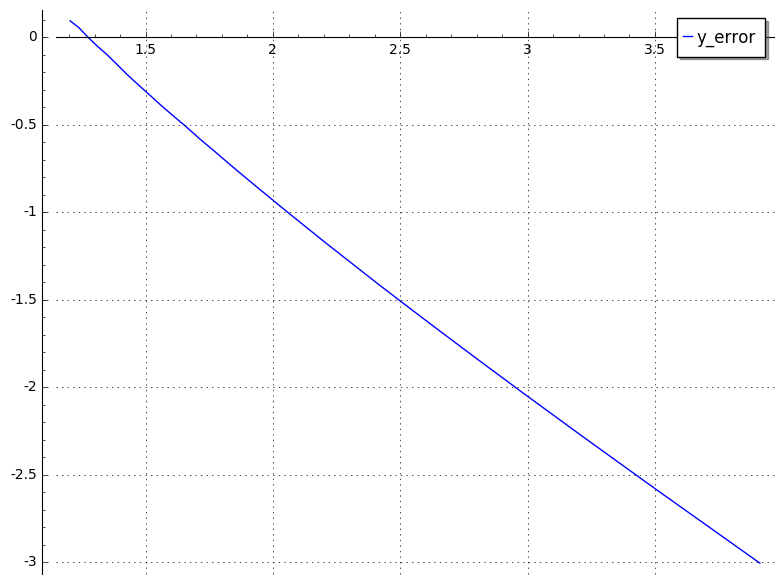
\includegraphics[width=0.4 \textwidth]{diff_eq_y_error.png}

Из них незатруднительно видеть, что метод имеет первый порядок ошибки.

\end{document}
